Based on the experiences made for \cite{preibisch2014efficient, schmid2015real}, this section will discuss results obtained with \gearshifft{} on various hardware in order to showcase the capabilities of \gearshifft{}. We will assume the motivation of a developer seeking to optimize the use of FFTs in the context of the aforementioned publications, i.e. 3D real-to-complex transforms with contiguous single-precision input data. If not stated otherwise, this is the transform type assumed for all illustrations hereafter. 
%
Expeditions into other use cases will be made where appropriate. The curious reader may rest assured that a more comprehensive study is possible with \gearshifft{}, however the mere multiplicity of all possible combinations and use cases of FFT render it neither feasible nor practical to discuss all of them here.

For this study, we will concentrate on three modern and current FFT implementations available free of charge: \fftw{} ($3.3.5$, on x86 CPUs), \cufft{} ($8.0.44$, on \nvidia{} GPUs) and \clfft{} ($2.12.2$, on x86 CPUs or \nvidia{} GPUs). We consider this the natural starting point of developers beyond possible domain specific implementations. It should be noted, that this will infer not only a study in terms of hardware performance, but also how well the APIs designed by the authors of \fftw{}, \clfft{} and \cufft{} can be used in practice. 

\subsection{Experimental Environment}
\label{ssec:env}

The results presented in the following sections were collected on three hardware installations:
%
\begin{table}[tbp]
  \centering
  \caption{Benchmark Hardware}
  \label{tab:hardware}
  \begin{tabular}{lllll}
    \toprule
                        & \multicolumn{2}{c}{\textbf{Taurus}}           & \textbf{Hypnos}           & \textbf{Islay}                                  \\
                        & \multicolumn{2}{c}{HPC Cluster \cite{taurus}} & HPC Cluster \cite{hypnos} & Workstation                                     \\
    \midrule
    \textbf{CPU family} & Haswell Xeon                                  & Sandybridge Xeon          & Haswell Xeon           & Haswell Xeon           \\
    \textbf{CPU model } & $2{\times}$ E5-2680 v3                        & $2{\times}$ E5-2450       & $2{\times}$ E5-2603 v3 & $2{\times}$ E5-2640 v3 \\
    \textbf{RAM       } & \SI{64}{\gibi\byte}                           & \SI{48}{\gibi\byte}       & \SI{64}{\gibi\byte}    & \SI{64}{\gibi\byte}    \\
    \textbf{GPU family} & Tesla                                         & Tesla                     & Tesla                  & GeForce                \\
    \textbf{GPU       } & 4x K80                                        & 2x K20x                   & 1x P100                & 1x GTX 1080            \\
    \textbf{GPU memory} & 4x \SI{12}{\gibi\byte}                        & \SI{6}{\gibi\byte}        & \SI{16}{\gibi\byte}    & \SI{8}{\gibi\byte}     \\
    \textbf{GPU driver} & $367.48$                                      & $367.48$                  & $367.48$               & $367.57$               \\
    \textbf{OS}         & RHEL $7.2$                                    & RHEL $7.2$                & Ubuntu $14.04.3$       & CentOS $7.2$           \\
    \bottomrule
  \end{tabular}
\end{table}
%
All systems presented in \cref{tab:hardware} will be used for the benchmarks in this section. Access was performed via a \texttt{ssh} session without running a graphical user interface on the target system. All measurements used the GNU compiler collection (GCC) version 5.3.0 as the underlying compiler. All used GPU implementations on \nvidia{} hardware interfaced with the proprietary driver and used the infrastructure provided by CUDA $8.0.44$ if not stated otherwise. 
After a warmup step a benchmark is executed five times. From this, the arithmetic mean and sample standard deviations are used for figures presented below. 

%TODO: why maximum size of transforms?

\subsection{Overhead of \gearshifft{}}
\gearshifft{} is designed to be a lightweight framework with a thin wrapper for the FFT clients, where the interface between back-end and front-end is resolved at compile-time. Performance indicators of each benchmark are collected and buffered to be processed after the last benchmark finished. For validation purposes, a \cufft{} standalone code \cite{gearshifft_github} was created that only measures the time to solution of a straightforward implementation of a round-trip FFT transform. Both invoke a warmup step and 5 repetitions of the benchmark. 

\cref{fig:verify_cufft} indicates a constant, almost zero overhead effect of \gearshifft{}.
However, the first benchmark run in \cref{fig:tts_verify_b} shows a difference of \SI{5}{\percent}. For reliable statistics it is recommended to use at least 20 benchmark repetitions.
These effects are also caused by an insufficient warmup phase, which will be fixed in an upcoming \gearshifft{} version. 
Regarding the mean runtime differences all other benchmark iterations show no significant runtime impact and the conclusions drawn in the following subsections are based on differences which are much stronger than \SI{5}{\percent} runtime deviation.

\begin{figure}[!htbp]
\vspace{-1em}
  \centering
  \includegraphics[width=\textwidth]{figures/results_validate_cufft_legend.pdf}\vspace{-1em}
  \subfloat[1024-point FFT]{\includegraphics[width=0.45\textwidth]{figures/results_validate_cufft_a.pdf}\label{fig:tts_verify_a}}
  \hfill
  \subfloat[16777216-point FFT]{\includegraphics[width=0.45\textwidth]{figures/results_validate_cufft_b.pdf}\label{fig:tts_verify_b}}
  \caption{Comparison of runtimes of \gearshifft{} vs. standalone \cufft{}---while the standalone \cufft{} was executed 250 times, \gearshifft{} processed a file with 250 rows containing the same number for the FFT extent; real-to-complex, inplace, round-trip FFT, on a Taurus K80 node \cite{taurus}.}
  \label{fig:verify_cufft}
\end{figure}

\subsection{Time To Solution}
\label{ssec:tts}

We begin the discussion with the classical use case for developers that might be accustomed to small size transforms. As such, an out-of-place transform with \texttt{powerof2} signal shapes will be assumed. The memory volume required for this operation amounts to the real input array plus an equally shaped complex output array of the same precision.   

\begin{figure}[!htbp]
  \centering
  \includegraphics[width=\textwidth]{figures/results_tts_legend.pdf}\vspace{-1em}
  \subfloat[linear scale]{\includegraphics[width=0.45\textwidth]{figures/results_tts_a.pdf}\label{fig:tts_a}}
  \hfill
  \subfloat[log10-log2 scale]{\includegraphics[width=0.45\textwidth]{figures/results_tts_b.pdf}\label{fig:tts_b}}
  \caption{Time-to-solution for power-of-2 3D single-precision real-to-complex out-of-place forward transforms using \fftw{} (\mc{FFTW_ESTIMATE}) and \cufft{}. \cref{fig:tts_b} shows the same data as \cref{fig:tts_a} but in a log10-log2 scale.}
  \label{fig:tts}
\end{figure}

\cref{fig:tts} reports a comparison of runtime results of power-of-2 single-precision real-to-complex forward transforms from \fftw{} and \cufft{}. It is evident that given the largest device memory available of  \SI{16}{\gibi\byte}, the GPU data does not yield any points higher than \SI{8}{\gibi\byte}. \cref{fig:tts_a} shows that the oldest GPU generation used in this comparison yields the slowest results for input signals in the order of \SIrange{1}{2}{\gibi\byte}. All other and more recent GPU models supersede \fftw{} using all available cores a $2{\times}12\,\text{core}$ double socket Intel Haswell CPU. Any judgment on the superiority of \cufft{} over \fftw{} can be considered premature at this point, as \fftw{} was used with the \mc{FFTW_ESTIMATE} planner flag.

\begin{figure}[!htbp]
  \centering
  \includegraphics[width=\textwidth]{figures/results_plan_flags_legend.pdf}\vspace{-1em}
  \subfloat[time to solution]{\includegraphics[width=0.45\textwidth]{figures/results_plan_flags_a.pdf}\label{fig:plan_flags_a}}
  \hfill
  \subfloat[time for forward transform only]{\includegraphics[width=0.45\textwidth]{figures/results_plan_flags_b.pdf}\label{fig:plan_flags_b}}
  \caption{Time-to-solution for power-of-2 3D single-precision real-to-complex inplace forward transforms using \fftw{} (\mc{FFTW_ESTIMATE}, \mc{FFTW_MEASURE}, \mc{FFTW_WISDOM_ONLY}) and \cufft{}. \cref{fig:plan_flags_a} report the complete time to solution, whereas \cref{fig:plan_flags_b} is limited to the time spent for the execution of the forward transform only. Both figures use a log10-log2 scale.}
  \label{fig:fftw_plan_flags}
\end{figure}

\cref{fig:fftw_plan_flags} compares the time-to-solution to the actual time spent for the FFT operation itself. This illustration makes the cost and the benefit of higher planning flags than \mc{FFTW_ESTIMATE} obvious. \mc{FFTW_MEASURE} imposes a total runtime penalty of 1 to 2 orders of magnitude with respect to \mc{FFTW_ESTIMATE}. It however offers superior performance considering FFT execution time compared to \mc{FFTW_ESTIMATE}. To compare \mc{FFTW_ESTIMATE} or \mc{FFTW_MEASURE} to plans using \emph{wisdom} (\mc{FFTW_WISDOM_ONLY} rigor), we generated wisdom files with the \mc{fftw_wisdom} binary. \mc{fftw_wisdom} was run to precompute plans for a canonical set of sizes (powers of two and ten up to $2^{20}$) in \mc{FFTW_PATIENT} mode, which in all took about one day on Taurus \cite{taurus} using (see \cite{fftw_manual} for command line flag details):
\begin{lstlisting}[language=bash]
 \$ fftwf-wisdom -v -c -n -T 24 -o wisdomf 
\end{lstlisting}

As during plan creation, the \emph{wisdom} has to be loaded from disk only, the planning times for calling the planner with \mc{FFTW_WISDOM_ONLY} are drastically reduced and \cref{fig:plan_flags_b} shows that the user is rewarded by pure FFT runtimes of less than an order of magnitude for small signal sizes. Unexpectedly, the FFT runtimes become larger than those of \mc{FFTW_ESTIMATE} for input signal sizes of more than \SI{32}{\kibi\byte}, which apparently contradicts the \mc{FFTW_PATIENT} setting which should find better plans than \mc{FFTW_MEASURE}.
%
It must be emphasized that the planning times for \mc{FFTW_MEASURE} become prohibitively long and reach minutes for data sets in the Gigabyte range. This is a well-known feature of \fftw{} as the authors note in \cite{FFTW05}:
%
\begin{quote}
  ``In performance critical applications, many transforms of the same
  size are typically required, and therefore a large one-time cost is
  usually acceptable.''
\end{quote}
% 
\gearshifft{} allows to dissect this problem further and isolate the planning time only.
%
\begin{figure}[!tbp]
  \centering
  \includegraphics[width=\textwidth]{figures/results_plan_time_legend.pdf}\vspace{-1em}
  \subfloat[3D transforms]{\includegraphics[width=0.45\textwidth]{figures/results_plan_time_a.pdf}\label{fig:plan_time_a}}
  \hfill
  \subfloat[1D transforms]{\includegraphics[width=0.45\textwidth]{figures/results_plan_time_b.pdf}\label{fig:plan_time_b}}
  \caption{Time-to-plan for power-of-2 single-precision inplace real-to-complex forward transforms using \fftw{}, \cufft{} and \clfft{}. \cref{fig:plan_time_a} reports the complete time to plan for 3D transforms, whereas \cref{fig:plan_time_b} is limited to 1D transforms. ``None'' refers to the planning with \cufft{} as it does not support the plan rigor concept. Both figures use a log10-log2 scale.}
  \label{fig:plan_time}
\end{figure}
%
\cref{fig:plan_time} illustrates the problem to its full extent. \mc{FFTW_MEASURE} consumes up to 3-4 orders of magnitude more time to produce a plan than a standard (GPU based libraries) or \mc{FFTW_ESTIMATE} based planner call especially for large input shapes, see \cref{fig:plan_time_a}. We compare the 3D planning with its counterpart in 1D (see \cref{fig:plan_time_b}). It is important to note that \fftw{} planning in 1D appears to be very time consuming as the \mc{FFTW_MEASURE} curve is very steep compared to \cref{fig:plan_time_a}. At input sizes of \SI{128}{\mebi\byte} in 1D, the planning phase exceeds the duration of \SI{100}{\second}. In practice, this imposes a challenge on the client to the \fftw{} API. Not only is the time to solution affected by this behavior which is a crucial quantity in FFT-heavy applications. Moreover, in an HPC environment the runtime of applications needs to be known before executing them in order to allow efficient and rapid job placement on compute resources. From another perspective, this asserts a development pressure on the developer interfacing with \fftw{} as she has to create infrastructure in order to perform the planning of \fftw{} only once and reuse the resulting plan as much as possible. Furthermore, based on these observations of \cref{fig:fftw_plan_flags} and \cref{fig:plan_time} weighing plan time versus execution time, it becomes more and more unclear for a user of \fftw{} which plan rigor to use in general.

\subsection{Comparing CPU versus GPU runtimes}
\label{ssec:cpu_vs_gpu}

The last section finished by discussing a design artifact, that the \fftw{} authors introduced in their API and which other FFT libraries adopted. Another important question typically asked is if GPU accelerated FFT implementations are really faster than their CPU equivalents. Although this question cannot be answered comprehensively in our study, we would like to point out several aspects of it. First of all, modern GPU are connected via the PCIe bus to the host system in order to transfer data, receive instructions and to be supplied with power. This imposes a severe bottleneck to data transfer and is sometimes neglected during library design. Therefor, the time for data transfer needs to be accounted for or removed from the measurement. \gearshifft{}s results data model offers access to each individual step of a transformation, see \cref{fig:framework}. With it, it is possible to isolate the time for the FFT transform only.

\begin{figure}[!tbp]
  \centering
  \includegraphics[width=\textwidth]{figures/results_r2c_fwd_legend.pdf}\vspace{-1em}
  \subfloat[3D transforms]{\includegraphics[width=0.45\textwidth]{figures/results_r2c_fwd_a.pdf}\label{fig:r2c_fwd_a}}
  \hfill
  \subfloat[1D transforms]{\includegraphics[width=0.45\textwidth]{figures/results_r2c_fwd_b.pdf}\label{fig:r2c_fwd_b}}
  \caption{Time for computing power-of-2 single-precision real-to-complex forward transforms using the 3D API (\cref{fig:r2c_fwd_a}) and the 1D API \clfft{} (\cref{fig:r2c_fwd_b}). Both figures use a log10-versus-log2 scale. Curves on the Intel E5-2680v3 based node were obtained with \fftw{}, the data on Nvidia GPUs was obtained with \cufft{}.}
  \label{fig:r2c_fwd}
\end{figure}

\cref{fig:r2c_fwd} shows the runtime spent for computing the forward FFT for real single precision input data. This illustration is a direct measure for the quality of the implementation and the hardware underneath. For the 3D case in \cref{fig:r2c_fwd_a}, we see that at the time of writing, \fftw{} on a double socket Haswell Intel Xeon E5 CPU provides very compelling performance if the input data is not larger than \SI{1}{\mebi\byte}. Above this limit, the GPU implementations offer a clear advantage by up to one order of magnitude. The current Pascal generation GPUs used with \cufft{} provide the best performance, which does not come by surprise as both cards are equipped with GDDR5X or HBM2 memory which are clearly beneficial for an operation that yields low computational complexity such as the FFT, see \cref{sec:motivation}. In the 1D case of \cref{fig:r2c_fwd_b}, the same observations must be made with even more certainty. The cross-over of \fftw{} and the GPU libraries occurs at an earlier point of \SI{64}{\kibi\byte}.  

Another observation in \cref{fig:r2c_fwd_a} is that the general structure of the runtime curves of GPU FFT implementations follows an inverse roofline curve \cite{williams2009roofline}. That is for input signals smaller than the roofline turning point at \SI{1}{\mebi\byte} the FFT implementation appears to be of constant cost, i.e. to be compute bound. Above the aforementioned threshold, the implementation appears to be memory bound and hence exposes a linear growth with growing input signals which corresponds to the $\mathcal{O}(n \log n)$ complexity observed in \cref{sec:motivation} and validates the considerations of algorithmic complexity therein as well. 

It is interesting to see that \cufft{} performance curves apparently follow a roofline like shape the best, whereas \fftw{} does not - most of all in \cref{fig:r2c_fwd_b}. We note that \gearshifft{} benchmark data could be well suited for creating roofline plots. However, the output data is currently not as detailed to produce comprehensive roofline graphs as discussed in \cite{ofenbeck2014applying} as hardware details (e.g. number of flops per cycle, number of flops per byte etc) are not contained. We would like to potentially address this issue in a future development of \gearshifft{} as this offers a unique chance to learn more about the capabilities and efficiency of the used implementation on the given hardware. 

Finally, it is not to our surprise that the \clfft{} results reported in \cref{fig:r2c_fwd} cannot be considered optimal. As we executed \clfft{} on Nvidia hardware interfacing with the OpenCL runtime coming with CUDA and interfaced to the Nvidia proprietary driver, OpenCL performance can not be considered a first-class citizen in this environment. Only in \cref{fig:r2c_fwd_b}, the \clfft{} runtimes are below those of \fftw{}. These experiments should be repeated on AMD hardware where the OpenCL performance is expected to be better.
 
\subsection{Non-power-of-2 transforms}
\label{ssec:nonpowerof2}

In a lot of conversations, the hypothesis is still often communicated, that input signals should be padded to power-of-2 shapes in order to achieve the highest possible performance. With \gearshifft{}, we can now probe the availability and quality of the common mathematical approaches across many FFT libraries. 

\begin{figure}[!tbp]
  \centering
  \includegraphics[width=\textwidth]{figures/results_non_power_of_2_legend.pdf}\vspace{-1em}
  \subfloat[Time for FFT]{\includegraphics[width=0.45\textwidth]{figures/results_non_power_of_2_a.pdf}\label{fig:non_power_of_2_a}}
  \hfill
  \subfloat[Time to Solution]{\includegraphics[width=0.45\textwidth]{figures/results_non_power_of_2_b_total.pdf}\label{fig:non_power_of_2_b}}
  \caption{Time for computing single-precision real-to-complex forward transforms using the 3D API \cref{fig:non_power_of_2_a} and the time to solution \cref{fig:non_power_of_2_b}. Both figures use a log10-versus-log2 scale.}
  \label{fig:non_power_of_2}
\end{figure}

Even though our findings in \cref{fig:non_power_of_2} are restricted to \fftw{} and \cufft{} for the sake of simplicity, the figure shows that this urban myth of padding for a power-of-2 to achieve better performance can be falsified to some extent. Clearly, power-of-2 transforms are the fastest among the three categories we chose. \cref{fig:non_power_of_2_a} illustrates that \fftw{} is able to offer almost identical performance for different input signal shape types across a very wide range of input signal volumes. This however comes at the expense of long planning times, which make it no match for the GPU based FFT library, see \cref{fig:non_power_of_2_b}. The situation is not so clear for \cufft{}. For large input signals, a FFT runtime difference of up to one order of magnitude on the K80 and the P100 can be observed (\cref{fig:non_power_of_2_a}) but the time to solution converges to a common limit due to planning and transfer penalties (\cref{fig:non_power_of_2_a}). For small input signal sizes, the plain FFT performance of the K80 is even superior to the P100 (\cref{fig:non_power_of_2_a}). In terms of time to solution, \cufft{} on the K80 is well ahead of the P100 for \mc{powerof2} inputs. For anything else, both GPUs offer comparable performance.

We conclude for a large range of input signal sizes between $\SIrange[exponent-base=2]{e-10}{e7}{\mebi\byte}$, a padding to power-of-2 might be justified when using \cufft{} if enough memory is available on the device. For \fftw{}, non-\mc{powerof2} signals can be padded at signal sizes above $\SI[exponent-base=2]{e-3}{\mebi\byte} = \SI{128}{\kibi\byte}$.    

\subsection{Data Types}
\label{ssec:data_types}

It is a common practice that complex-to-complex transforms are considered more performant than real-to-complex transforms. So, in order to transform a real input array, a complex array is allocated and the real part of each datum is filled with the signal. The imaginary part of each datum is left at $0$.

\begin{figure}[!tbp]
  \centering
  %
\includegraphics[width=\textwidth]{figures/results_r2c_vs_c2c_legend.pdf}
  \subfloat[single precision]{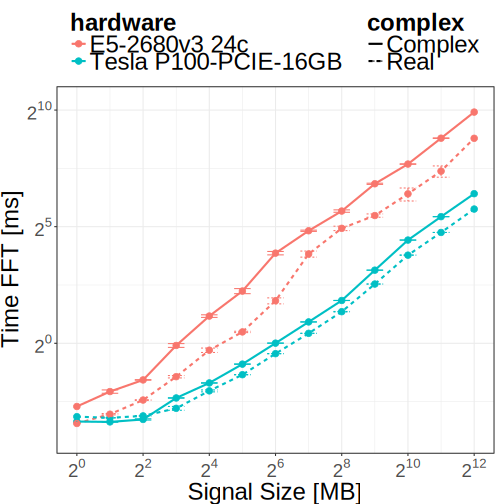
\includegraphics[width=0.45\textwidth]{figures/results_r2c_vs_c2c_a.pdf}\label{fig:r2c_vs_c2c_a}}
  \hfill
  \subfloat[real-to-complex]{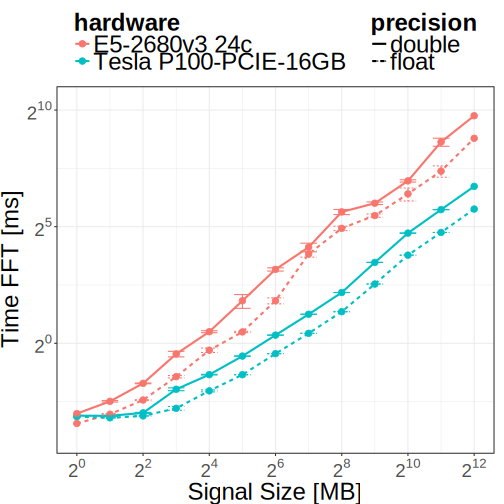
\includegraphics[width=0.45\textwidth]{figures/results_r2c_vs_c2c_b.pdf}\label{fig:r2c_vs_c2c_b}}
  \caption{Time for computing a forward FFT transform using 3D power-of-2 input signals using \fftw{} and \cufft{} on respective hardware versus the number of elements in the input signal. \cref{fig:r2c_vs_c2c_a} computes a real-to-complex transform and compares it to a complex-to-complex transform for single precision input data, whereas \cref{fig:r2c_vs_c2c_b} shows a real-to-complex transform for either single or double precision. Both figures use a log2-versus-log2 scale.}
  \label{fig:r2c_vs_c2c}
\end{figure}

\cref{fig:r2c_vs_c2c} restricts itself to larger signal sizes in order to aid the visualization. Note that in \cref{fig:r2c_vs_c2c_a}, a data point at the same number of elements of the input signal does have different size in memory. \fftw{} exposes a factor of 2 and more of runtime difference for signals larger than $2^{15}$ elements comparing real and complex input data types in \cref{fig:r2c_vs_c2c_a}. Below this threshold, the performance can be considered identical except for very small input signals although real FFTs always remain faster than complex ones. The situation is different for \cufft{}, where the overall difference is smaller in general. In the compute bound region of \cufft{} (below $2^{19}$ elements), complex transforms perform equally well than real transforms given the observed uncertainties. In the memory bound region (above $2^{19}$ elements), real transforms can be a factor of 2 ahead of complex ones which is clearly related to twice the memory accesses.    

 \cref{fig:r2c_vs_c2c_b} tries to answer the question, what gain can be expected if double precision is not needed for computing an FFT. On the high grade server GPU, the \nvidia{} Tesla P100, the performance difference remains around $2{\times}$ in the memory bound region due to double the memory bandwidth required. The results for \fftw{} vary more around \numrange{1.5}{2.5} fold regressions between single and double precision inputs across a wider input signal range. 

